% ------------------------------------------------------------------
\renewcommand{\thisweek}{MATH327 Week 11}
\renewcommand{\moddate}{Last modified 7 May 2021}
\setcounter{section}{11}
\setcounter{subsection}{0}
\phantomsection
\addcontentsline{toc}{section}{Week 11: Synthesis and broader applications}
\section*{Week 11: Synthesis and broader applications}
\subsection{\label{sec:MonteCarlo}Monte Carlo importance sampling}
Last week we wrapped up our discussion of the mean-field approximation to the Ising model by comparing some of its predictions against results from numerical computations for systems in $d \geq 3$ dimensions where no exact solution is known.
These numerical results may have come as a surprise given the statement at the end of \secref{sec:Ising} that numerically evaluating the Ising model partition function even for tiny systems with $N \sim 1000$ spins is far beyond the capabilities of existing or foreseeable supercomputers.
To quantify `tiny', consider that $N \sim 1000$ would correspond to a $10\times 10\times 10$ lattice in three dimensions or a $6\times 6\times 6\times 6$ lattice in four dimensions, both very far from the thermodynamic limit of interest for phase transitions.

The key is that practical numerical computations do not perform a `brute-force' evaluation of every single micro-state that is summed over in the formal definition of the partition function (and hence in the expectation values that we have derived from the partition function).
Instead, they proceed by (pseudo-)randomly selecting (or \textbf{sampling}) a small subset of those micro-states, and using this subset to compute results for the average energy, magnetization, and other thermodynamic quantities.
The law of large numbers allows us to treat these averages as controlled approximations to the true ensemble expectation values.

As we saw in the computer project, such numerical calculations employ pseudo-random numbers rather than complete randomness, which allows them to be reproducible up to very high precision by different people using different computers.
Due to the role of randomness, these numerical approaches have become known as \textbf{Monte Carlo} methods, based on a whimsical reference to the famous gambling centre in Monaco.
Monte Carlo methods are crucial in statistical physics because they are applicable even to the interacting systems introduced last week, where there are no longer dramatic simplifications from factorization.

An intuitive illustration of how Monte Carlo methods work is provided by using them to numerically evaluate integrals.
The idea is that the integral can be numerically approximated by evaluating its integrand at randomly sampled points in the integration domain, and normalizing by the number of samples.
A simple example is to compute
\begin{align*}
  \int_{-1}^1 dx \int_{-1}^1 dy \ H\!\left(1 - \left\{x^2 + y^2\right\}\right) & = \pi \qquad &
  H(r) & = \left\{\begin{array}{l}1 \qquad \mbox{for } \ r \geq 0 \\
                                  0 \qquad \mbox{for } \ r < 0\end{array}\right. ,
\end{align*}
which is just the area of a disk with radius $R = 1$, in a square integration domain with area $4$, as shown below.
Since the integrand is either $0$ or $1$ for each randomly sampled point in that domain, simply counting the fraction of the $S$ samples that lie in the disk provides a numerical determination of $\pi$, with a \textit{statistical uncertainty} that vanishes $\sim 1 / \sqrt{S}$.
In just a few minutes, \href{https://github.com/daschaich/MATH327_2021/blob/master/lecture_notes/week11_pi.py}{this Python code} predicts $\pi = 3.14155 \pm 0.00024$ purely from the statistics of pseudo-random numbers.

\begin{center}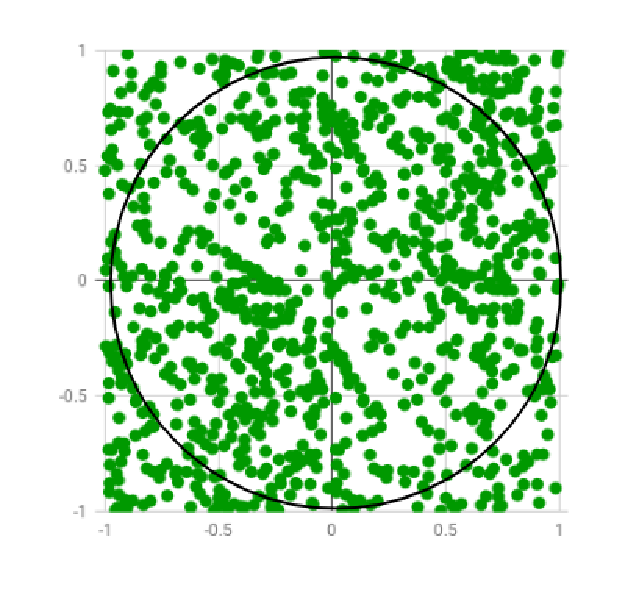
\includegraphics[width=0.6\textwidth]{figs/week11_pi.pdf}\end{center}

Of course, Monte Carlo integration is an extremely inefficient way to determine $\pi$.
These numerical methods are most useful when analytic solutions are not available, and especially for very high-dimensional integrals such as partition functions of statistical systems.
State-of-the-art research in theoretical physics routinely uses Monte Carlo methods to numerically evaluate billion-dimensional integrals.

Switching back to the language of statistical ensembles, there are an enormous number of possible micro-states for any interacting systems of interest, only a vanishingly small fraction of which can be sampled in a reasonable amount of time.
Even if we put in the time to sample a trillion ($10^{12}$) micro-states of the tiny $N \sim 1000$ Ising systems considered above, this would account for only about one part in $10^{288}$ of the total $2^N \sim 10^{300}$ micro-states.
Even worse, as $N$ increases the number of possible Ising model micro-states grows exponentially quickly, $2^N$, and each micro-state takes more work to sample.
For a concrete example, \href{https://arxiv.org/abs/1502.07613}{this research publication} from 2015 includes a calculation with $N \sim 10^9$ that was only able to sample $\sim 10^4$ out of roughly $2^{10^9} \sim 10^{300{,}000{,}000}$ micro-states. % N=64^5~1e9 and log_10(2^(64^5))~3e8

For sufficiently high temperatures, our consideration of the disordered phase of the Ising model in \secref{sec:Ising_phases} suggests that randomly sampling even such a tiny fraction of the micro-states would still suffice.
All of those micro-states are equally probably in the infinite-temperature limit, where we would just need to consider enough samples $S$ to produce reasonably small statistical uncertainties $\sim 1 / \sqrt{S}$.
However, the low-temperature ordered phase is more challenging.
We saw that the large-scale behaviour of the system in this phase is dominated by a very small number of micro-states.
For sufficiently low temperatures, just the two degenerate ground states effectively determine the magnetization, with only exponentially suppressed corrections from higher-energy excited states.
As there is essentially no chance of randomly sampling either of those two ground states, the approach described above seems doomed to fail.

The cure is to carefully guide the procedure so that the probability of sampling a particular micro-state $\om_i$ is proportional to its probability $p_i \propto e^{-\be E_i}$, without introducing any bias.
This is known as \textbf{importance sampling}, since it preferentially samples the important micro-states that make the most significant contributions to the partition function and derived quantities.
As $\be \to \infty$ in the low-temperature phase, the probability of sampling the ground states would be exponentially enhanced, as desired.
As $\be \to 0$ in the high-temperature phase, there would be little change compared to the more straightforward approach described above, since all micro-states would become equally probable.

A challenge facing importance sampling is that the energies $E_i$ are not known in advance.
They are generally only computed for those few micro-states that are sampled.
An ingenious way to get around this challenge\footnote{This approach was developed in 1953 by \href{https://en.wikipedia.org/wiki/Nicholas_Metropolis}{Nick Metropolis}, \href{https://en.wikipedia.org/wiki/Arianna_W._Rosenbluth}{Arianna Rosenbluth}, \href{https://en.wikipedia.org/wiki/Marshall_Rosenbluth}{Marshall Rosenbluth}, \href{https://en.wikipedia.org/wiki/Augusta_H._Teller}{Mici Teller} and \href{https://en.wikipedia.org/wiki/Edward_Teller}{Edward Teller}.  In an infamous misfiring of alphabetical ordering, it remains widely known as the ``Metropolis algorithm'' even though Metropolis's role was providing specialized computing equipment rather than creating the algorithm itself.  In addition, the key contributions of Arianna Rosenbluth and Mici Teller were under-appreciated for many years.} is by incorporating the concept of Markov chains that we encountered all the way back in \secref{sec:diffusion}.
Recall that a Markov chain is a process in which the next micro-state to be sampled is chosen based on the micro-state currently under consideration, with no `memory' of any other micro-states that may already have been sampled.

Applying this to the Ising model, we can begin with any random spin configuration.
Randomly selecting one spin, $s_i$, we compute $\De E_i$, the change in the system's energy that would be caused by flipping $s_i \to -s_i$.
We then update the spin configuration by `accepting' this spin flip with probability
\begin{equation}
  \label{eq:MRTprob}
  P_{\text{accept}} = \mbox{min}\left\{1, e^{-\be \De E}\right\},
\end{equation}
which defines the next micro-state in the Markov chain.
Importantly, this new micro-state may be identical to the previous micro-state with probability $P_{\text{reject}} = 1 - P_{\text{accept}}$.
This is exactly what we would want in the zero-temperature limit where the ground state should dominate.
We then repeat this single-spin update procedure as many times as our computers can handle.

Digging into \eq{eq:MRTprob}, we can see that a spin flip that lowers the energy will always be accepted, since $\De E < 0 \implies e^{-\be \De E} > 1$.
The algorithm is therefore free to approach the minimum-energy ground state of the system.
If it is in the ground state, then any spin flip will increase the energy, $\De E > 0$, and will only be accepted with an exponentially suppressed probability $e^{-\be \De E} \to 0$ as $T = 1 / \be \to 0$, as desired.
More generally, if we consider two micro-states $\om_A$ and $\om_B$ with $E_A \leq E_B$, then the relative probabilities of moving between these two micro-states are
\begin{equation*}
  \frac{P(A \to B)}{P(B \to A)} = \frac{\mbox{min}\left\{1, e^{-\be(E_B - E_A)}\right\}}{\mbox{min}\left\{1, e^{-\be(E_A - E_B)}\right\}} = \frac{e^{-\be(E_B - E_A)}}{1} = \frac{e^{-\be E_B}}{e^{-\be E_A}},
\end{equation*}
confirming that the micro-states $\om_i$ will indeed be sampled with probabilities proportional to the Boltzmann factors $e^{-\be E_i}$ that quantify their importance.

You can find more information about this \textit{Metropolis--Rosenbluth--Teller} algorithm in Section~8.2 of Schroeder's \textit{Introduction to Thermal Physics} (reference~2 in the list of further reading on page~6), including a single-page annotated code applying it to the two-dimensional Ising model.
While this is the most famous and most widely used Monte Carlo algorithm in existence, it is far from the only one.
There is an enormous amount of ongoing research developing, optimizing and applying more elaborate Monte Carlo methods to investigate topics throughout the mathematical sciences and beyond.
In \secref{sec:broad} we will briefly look at some of these broader applications.
First, there is another important concept to introduce, called universality, which helps to explain why interacting statistical systems are so useful to apply to such a diverse range of scientific investigations.
% ------------------------------------------------------------------



% ------------------------------------------------------------------
\subsection{Universality}
In \secref{sec:mean_field} we defined the critical exponent $b$ as the power governing the behaviour of the order parameter $\vev{m} \propto \left(T_c - T\right)^b$ as the temperature $T$ approaches the critical temperature $T_c$ of the second-order phase transition.
In addition to being an important feature characterizing any given phase transition, it was discovered during the twentieth century that precisely the same critical exponents turn out to govern the behaviour of phase transitions that we initially would not have expected to have any connection.
For example, the critical exponent $b \approx 0.32$ for the three-dimensional Ising model magnetization mentioned last week also appears at the phase transition where an interacting (non-ideal) gas transforms into a liquid,
\begin{align*}
  \frac{1}{\rho_{\text{gas}}} - \frac{1}{\rho_{\text{liquid}}} & \propto \left(T_c - T\right)^b &
  b & \approx 0.32,
\end{align*}
where $\rho$ is the density of the atoms, which are equal for the two phases at the transition.\footnote{We're not covering the liquid--gas transition in this module.  If you are curious about it, you can find a discussion in Section~5.1 of David Tong's \href{https://www.damtp.cam.ac.uk/user/tong/statphys.html}{\textit{Lectures on Statistical Physics}} (reference~1 in the list of further reading on page~6).}

This is not simply a numerical coincidence, but an example of an amazing phenomenon is known as \textbf{universality}.
In essence, universality states that the specific details of interacting statistical systems become irrelevant close to critical points at which phase transitions occur.
It doesn't matter whether we are considering a three-dimensional lattice of Ising spins or a liquid such as water---the behaviour of both systems is governed by the same set of critical exponents (known as their \textit{universality class}).

The detailed mathematics underlying universality is well beyond the scope of this module.
Important contributions to its development were made by \href{https://en.wikipedia.org/wiki/Leo_Kadanoff}{Leo Kadanoff} and \href{https://en.wikipedia.org/wiki/Kenneth_G._Wilson}{Ken Wilson}, among many others.
The purpose of this section is just to quickly introduce the concept and emphasize that universality causes the same large-scale behaviour to appear in the vicinity of critical points even for systems that initially may seem completely different.
This independence of the details of the system helps to explain the power of even simple interacting statistical systems such as the Ising model, and their applicability in so many different domains.
% ------------------------------------------------------------------



% ------------------------------------------------------------------
\subsection{\label{sec:broad}Broader applications}
In this section we will continue to provide quick introductions rather than detailed derivations, considering a few ways in which the concepts and tools of statistical physics are applied beyond the mathematical sciences.
The cases considered here are far from exhaustive, and many more examples may become apparent now that we have gained familiarity with the underlying statistical methods and perspectives.

\subsubsection*{Voter models}
Sociology is one domain where the applicability of statistical physics may be unexpected.
Despite (possible) expectations, there is a diverse and active field of ``sociophysics'', which uses the statistical physics concepts and tools that we have been learning about to describe various aspects of social and political behavior.\footnote{For a review, see Serge Galam, \href{https://liverpool.idm.oclc.org/login?url=http://dx.doi.org/10.1007/978-1-4614-2032-3}{\textit{Sociophysics: A Physicist's Modeling of Psycho-political Phenomena}} (2012).}

A particular branch of sociology where connections to statistical physics may be more apparent is the field of opinion formation, where so-called \href{https://en.wikipedia.org/wiki/Voter_model}{voter models} have been widely used since the 1970s, and have proved capable of capturing outcomes of elections.
Voter models are interacting statistical systems not too different from the Ising model, where spin degrees of freedom that we have been working with are interpreted as voters' opinions on a certain topic.
For example, support for a proposal or candidate can be represented as $s_i = +1$, while opposition would be $s_i = -1$.
Just like the interactions in the Ising model encourage spins to align with each other, voter models build in a tendency for voters to align (i.e., agree) with the majority of other voters they interact with.

There are many generalizations that can then be incorporated to better describe the outcome of polls and elections.
A simple extension would be to allow voters to be neutral or indifferent to the question, represented as $s_i = 0$.
Similarly, the strength of a voter's commitment to their opinion can be modelled by extending the range of possible spin values,
\begin{equation*}
  s_i \in \left\{\cdots, -2, -1, 0, +1, +2, \cdots\right\}.
\end{equation*}

Another way to make voter models more realistic is to define them on more flexible \textit{graphs} rather than regular lattices.
The figure below (\href{https://doi.org/10.1073/pnas.1200709109}{source}) illustrates how such a graph can look for a two-state system with $s_i \in \left\{-1, +1\right\}$ coloured red and blue.
As in everyday experience (and inspired by social networks), different voters can have connections with different numbers of other voters, who do not need to be nearest neighbours.
In this particular investigation, network connections between disagreeing voters are probabilistically severed, and transitions are observed between a phase in which one of the opinions becomes the consensus, or all connections are severed between the two groups with differing opinions.

\begin{center}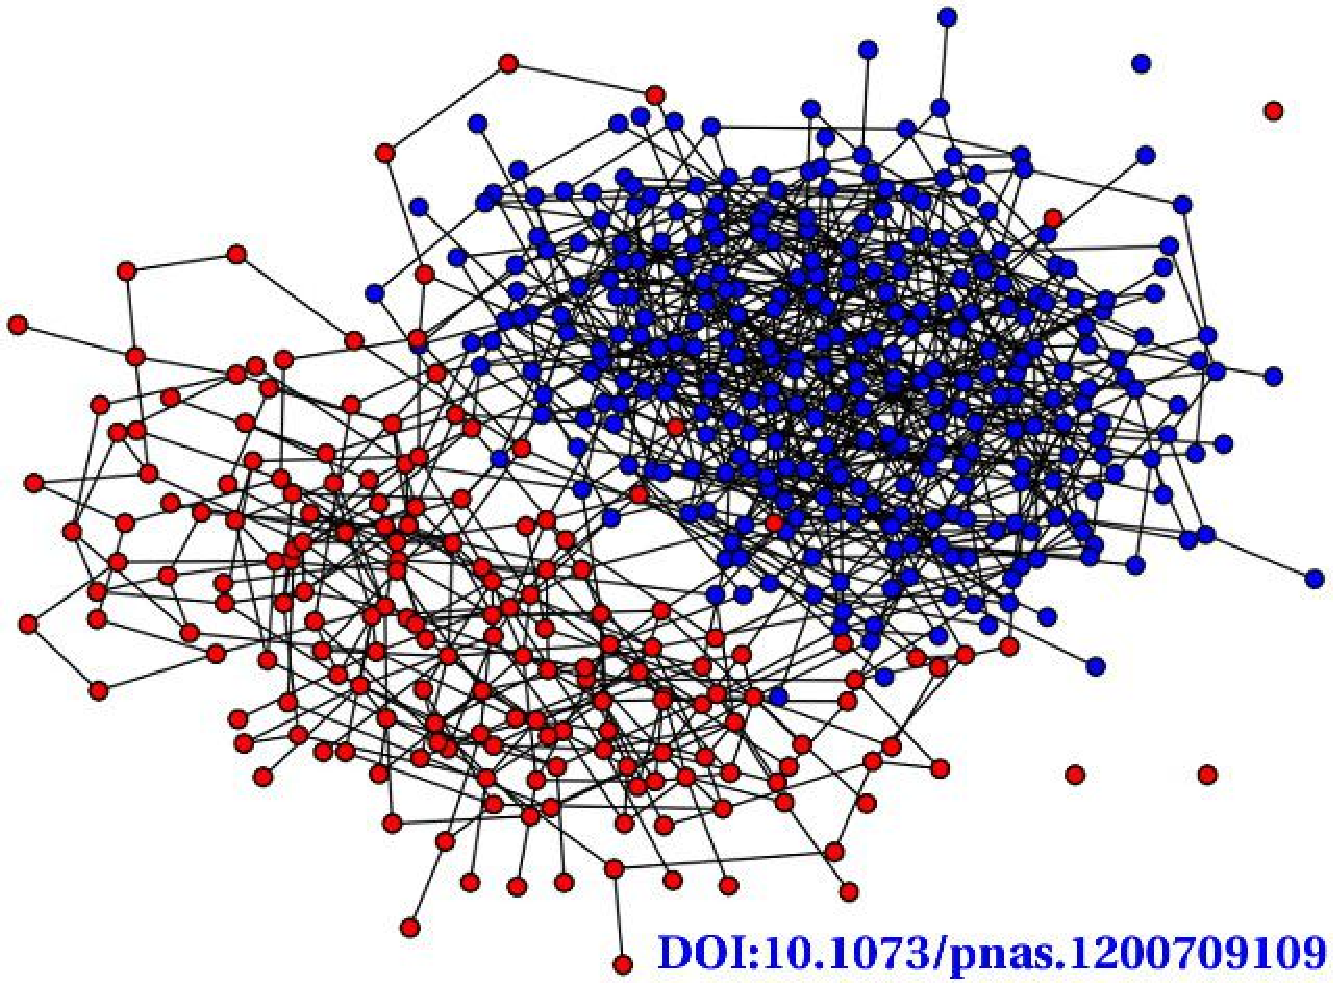
\includegraphics[width=0.7\textwidth]{figs/week11_voter.pdf}\end{center}

Simpler studies that don't involve severing connections have observed a similar consensus phase occurring once an opinion reaches a critical concentration.
Remarkably, this was found to be described by a second-order phase transition in the universality class of the two-dimensional Ising model.
Another outcome possible in certain voter models is a ``stable non-consensus'' phase, in which the two opinions persist indefinitely, each one held by a `cluster' of aligned voters who interact mainly with each other rather than with voters holding the opposite opinion.
These investigations are described by Alexander Balankin et al., ``\href{https://doi.org/10.1016/j.physleta.2016.12.001}{Ising percolation in a three-state majority vote model}'' (2016).

\subsubsection*{Epidemiology}
A particularly topical application of interacting statistical systems is to model the spread of diseases in populations, something most of us may have seen in the news over the past fifteen months.
As in the case of voter models, the degrees of freedom under consideration are again individuals, whose interactions with each other allow infection to spread to those who are susceptible.
A Monte Carlo calculation of the sort described in \secref{sec:MonteCarlo} can then be used to model how many people may be infected as time passes, guided by data on typical movement and contacts.

The figure below comes from \href{https://www.washingtonpost.com/graphics/2020/world/corona-simulator/}{an over-simplified simulation} provided by the \textit{Washington Post} to illustrate these concepts.
Here individuals are modeled simply as a gas of interacting particles in two dimensions, and various ways of restricting their motion are used to explore the likely effects of measures such as quarantines and social distancing.
By coincidence, the scale of this simulation, which considers a population of just $200$ people, is comparable to the first importance sampling Monte Carlo calculation carried out in 1953 as a first application of the Metropolis--Rosenbluth--Teller algorithm.
\href{https://en.wikipedia.org/wiki/Equation_of_State_Calculations_by_Fast_Computing_Machines}{That historic investigation} computed the pressure (i.e., equation of state) for $224$ interacting particles in a two-dimensional `volume'.
At the time, this required several days of computing time on a state-of-the-art machine; now these sorts of calculations are easily done on a smartphone.

\begin{center}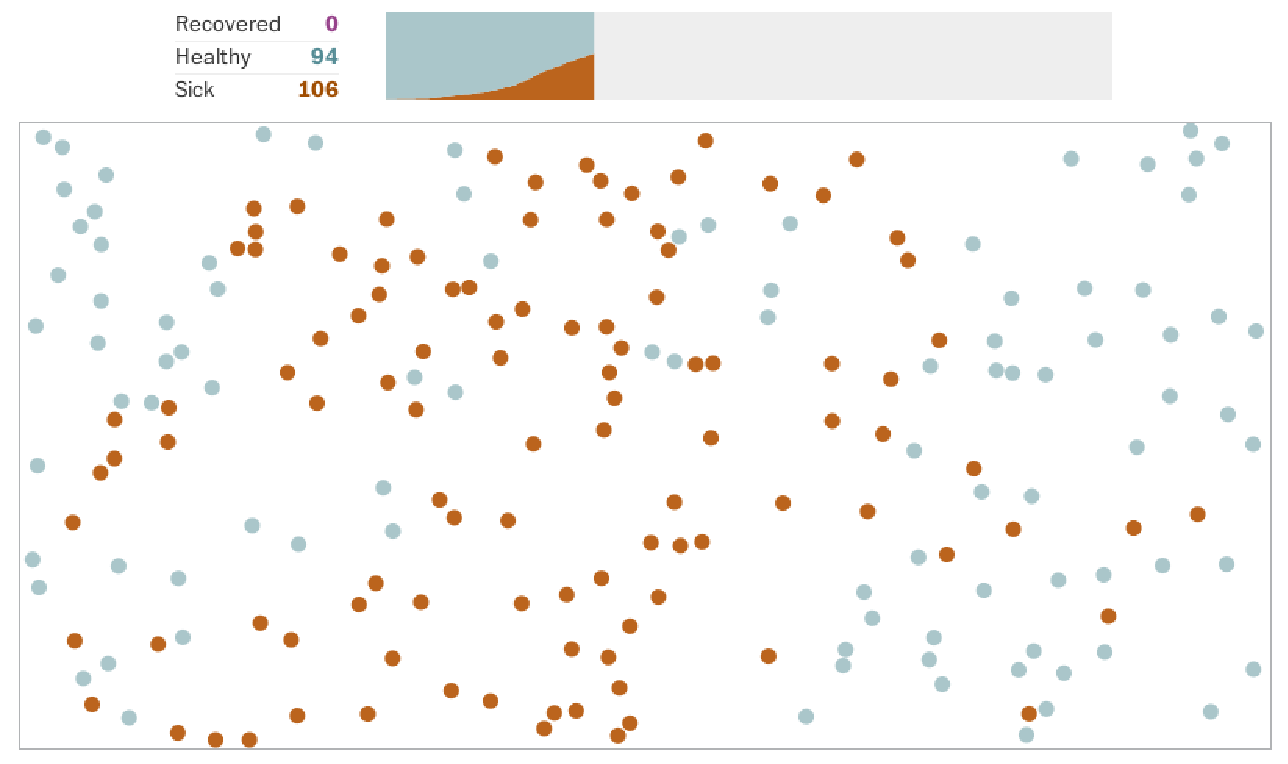
\includegraphics[width=0.8\textwidth]{figs/week11_epidemic.pdf}\end{center}

Larger-scale and more realistic versions of these epidemiological simulations provide important input into government deliberations regarding what restrictions (such as lockdowns) would be most beneficial to reduce the spread of disease, and how long such restrictions may need to be maintained.
Rather than investigating a phase transition, the goal is to quantify likely effects of restrictions (or of the absence of restrictions).
As described in \secref{sec:LLN}, the numerical experiments are therefore repeated many times with different sequences of pseudo-random numbers.
This produces an ensemble of possibilities from which the likely outcomes of various interventions can be inferred.

\subsubsection*{Flocking}
Let's conclude our quick glimpses of some broader applications of statistical physics by considering another biological example, where interacting statistical systems are used to model the large-scale collective motion of certain groups of animals.
The image below (from Marcus Woo, ``\href{https://www.sciencemag.org/news/2014/07/how-bird-flocks-are-liquid-helium}{How bird flocks are like liquid helium}'', \textit{Science}, 27 July 2014) illustrates the so-called flocking behaviour of large groups of starlings, which fly through the sky in surprisingly tight coordination.
This same sort of behaviour is also seen in schools of fish, swarms of insects, and even crowds of humans.

\begin{center}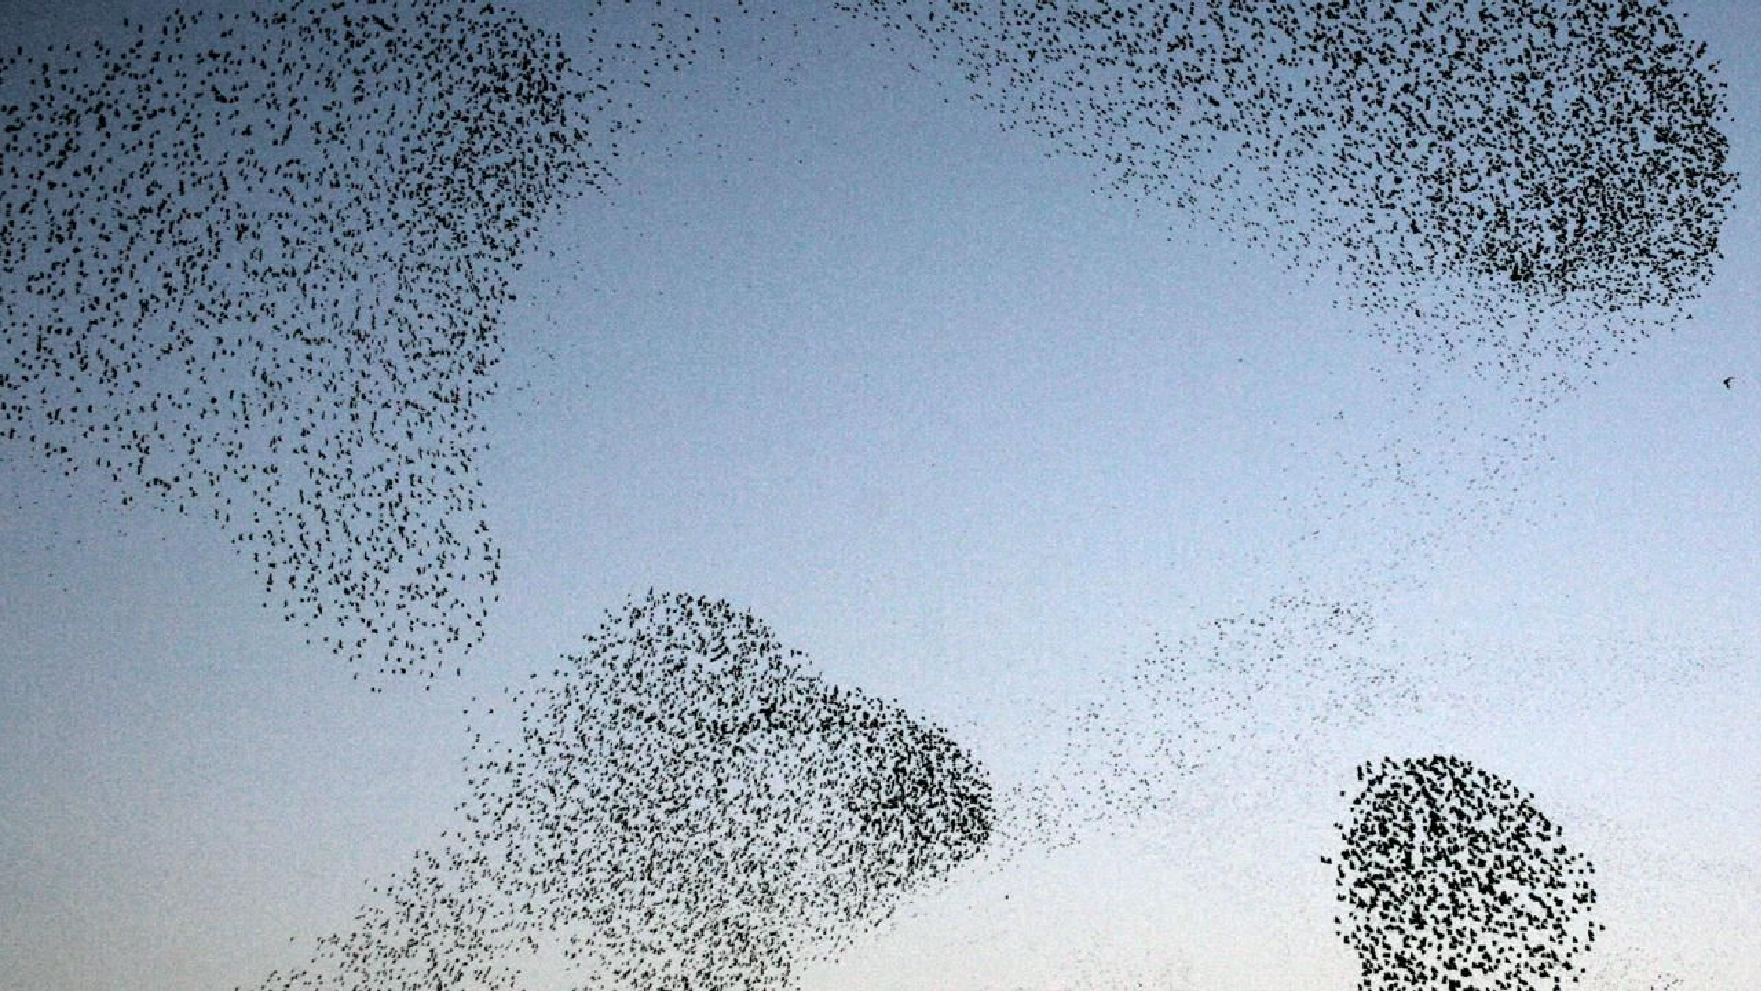
\includegraphics[width=0.8\textwidth]{figs/week11_flock.pdf}\end{center}

Many models based on interacting statistical systems have been (and continue to be) developed to describe this emergent collective behaviour.
A particularly simple and widely studied \href{https://en.wikipedia.org/wiki/Vicsek_model}{example} was introduced in 1995.
It proposes that each particle (i.e., bird) will interact with others near to it, and this interaction will encourage it to move in the same direction as its neighbours, in much the same way that the nearest-neighbour interactions in the Ising model encourage its spins to align.

This model exhibits a transition between two distinct phases.
When there is a low density of particles, there are relatively few interactions and the particles' motion is disordered, with no formation of flocks or swarms.
At high densities, in contrast, large-scale collective motion appears, based solely on the interactions between the individual particles in the system.
These two regimes turn out to be separated by a first-order phase transition, with a discontinuity (in the thermodynamic limit) in an order parameter related to the average angle of flight.
In addition, as the critical density is approached, flights in the disordered phase exhibit anomalous super-diffusion like that investigated in the computer project.
% ------------------------------------------------------------------



% ------------------------------------------------------------------
\subsection{Wrap-up recap and synthesis}
We have covered a lot of ground in this module, building on foundations from probability to develop and apply the core concepts of statistical physics.

%Learning outcomes
% * Demonstrate understanding of the micro-canonical, canonical and grand-canonical ensembles, their relation and the derived concepts of entropy, temperature and particle number density.
% * Understand the derivation of the equation of state for non-interacting classical and quantum gases.
% * Demonstrate numerical skills to understand diffusion from an underlying stochastic process.
% * Know the laws of thermodynamics and demonstrate their application to thermodynamic cycles.
% * Be aware of the effects of interactions, including an understanding of the origin of phase transitions.

\TODO{Being written...}


% Statistical Physics is a core subject in Physics and a cornerstone for modern technologies. To name just one example, quantum statistics is informing leading edge developments around ultra-cold gases and liquids giving rise to new materials. The module will introduce foundations of Statistical Physics and will develop an understanding of the stochastic roots of thermodynamics and the sometimes-illusive properties of matter. After successfully completing this module students will understand statistical ensembles and related concepts such as entropy and temperature, will understand the properties of classical and quantum gases, will be know the laws of thermodynamics and will be aware of advanced phenomena such as phase transition. The module will also deliver key numerical skills for the description of macroscopic effects such as diffusion by an underlying stochastic process.
% ------------------------------------------------------------------
